\subsection{First Demo}
Primero habia un demo en el que habia un sistema de autosar bastante mas simple para el cual tuvimos que hacer varias cosas antes de arrancar, como hackearle el flexray y eso. Luego creamos un modelo en python que enviara datos por CAN. Despues de leer el stack de comunicacion de Autosar me di cuenta que habian varias cosillas que no tenian logica y al parecer el sw wstaba mal planteado. 

Tambien habla de que al comienzo creias que la version inical era la TC37x pero estando en este punto te toco hacer el modelado del microcontrolador.
\subsection{Use Cases}
Segun la documentacion del gateway, este gateway esta conectado de la sgte forma

\begin{figure}[!htb]
 \centering
 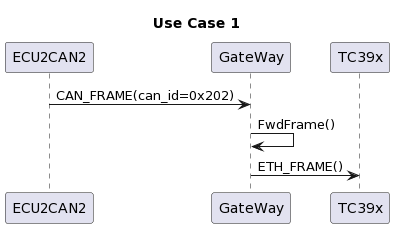
\includegraphics[width=0.5\textwidth]{img/GWUseCase1.png}
 \caption{Gateway Demo Use Case 1}
 \label{fig:gw-demo-uc1}
\end{figure}

\begin{figure}[!htb]
 \centering
 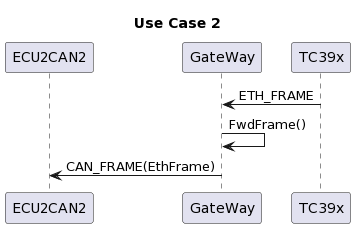
\includegraphics[width=0.5\textwidth]{img/GWUseCase2.png}
 \caption{Gateway Demo Use Case 2}
 \label{fig:gw-demo-uc2}
\end{figure}

Tonces lo primero que habia que hacer era tener algun tipo de componente que envie datos por el bus can y por ethernet para que sean recibidos por el 
Tonces lo primero que habia que hacer era leer el stack de comunicaciones de autosar y saber lo que el 
\subsection{Use Case 1}
En este Gateway hay una cierta cantidad de componentes que hay que modelar porque el software intenta comunicarse con ellos. Cogi el modelo que habia desarrollado en el caso anterior y le puse funcionalidades de Ethernet y de LIN (para un posterior uso) y lo conecte con el AURIX como se muestra en la figura \ref{fig:connections-diagram}

\begin{figure}[!htb]
 \centering
 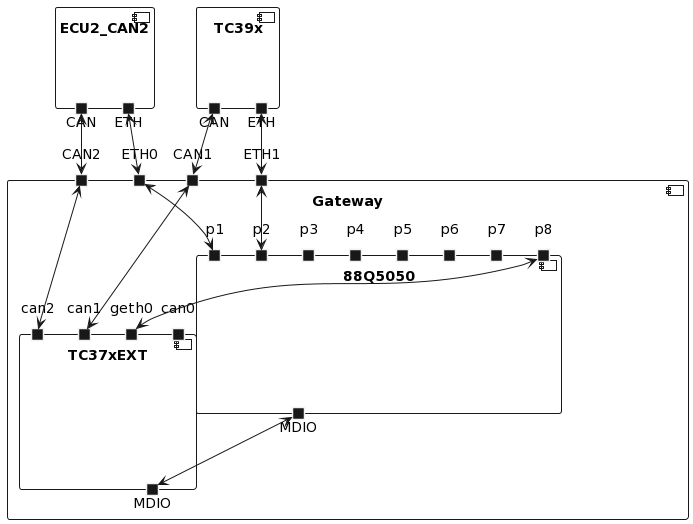
\includegraphics[width=\textwidth]{img/GWConnectionsDiagram.png}
 \caption{Gateway Connections Diagram}
 \label{fig:connections-diagram}
\end{figure}

Al comienzo no nos planteamos necesario modelar el switch pero luego nos dimos cuenta que el AURIX se intenta comunicar con el y sin sus respuestas no hay nada que funcione. Aqui les pones un UML de la secuencia de verificacion del switch. Resulta que los switches tienen un modo que se llama RMU que significa Remote management Unit y eso entra en una categoria que se llama Distributed Switch Architecture que permite que puedas controlar un switch con una cpu externa. En este caso se usa en la secuencia de inicializacion para tener acceso a los registros del switch. Para esto se ajusta el modo RMU desde los pines del MDIO y luego se mandan datos por ethernet en el puerto 8 (IMPORTANTE QUE SEA SOLO EL PUERTO 8) con un Tag especial de protocolo SNAP (SubNetwork A Protocol) (en este punto nos toco agregar support para los codigos SNAP en el modelo del microcontrolador) y luego se envia un arespuesta siguiendo el protocolo de Marvell. hasta aqui lo llevo yo el dia de hoy.

Luego muestras que envias un dato desde CAN con el id que es y que no funcionaba porque patata

\subsection{Use Case 2}

Ni idea que voy a poner aqui.